\documentclass[11pt]{article}
\usepackage{amsmath, fullpage, parskip, graphicx}

\begin{document}
\title{DS Coursework}
\author{Jacob Essex \\ s1040340}
\maketitle

\subsection*{Q1}

I assume that the starting time $(0,0)$ is some point before either of the first events for $p_1$ or $p_2$ occur. This is slightly more general than the notation used in some of the slides in which it is assumed that both of the first events have occurred. Should this actually be what is wanted then as the below graph is more general the point at which the first two events have occurred is $(1,1)$

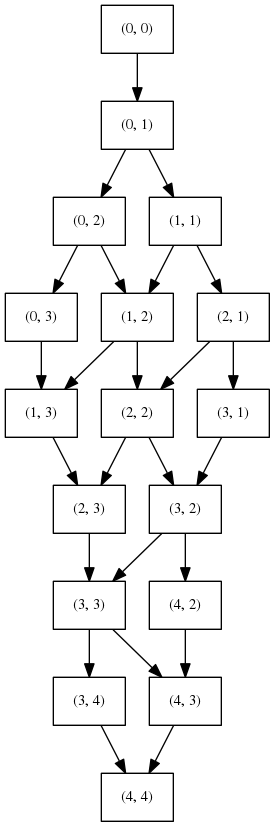
\includegraphics[width=0.3\textwidth]{q1_theory.png}


\subsection*{Q2}
To avoid starvation an algorithm needs to be fair (i.e. requests for a lock are honored in the order that they are made). This prevents starvation. A system that is liable to have starvation is one that always grants the request of the most recent request for a mutex over that of older requests.

\subsection*{Q3}

Data is transfered between nodes. This data is of fixed size and is represented using the following tuple
$$
(\text{sum of all p.f seen}, \text{max of all p.f seen}, \text{number of processors seen})
$$

The algorithm is as follows:

The root node sends a request to all children for the data. All children then send the request onwards to their children etc. This takes $O(n)$ time as there is a fixed message length in the word case the tree is a list where each node has $0$ or $1$ children.

Each leaf sends its $(p.f, p.f, 1)$ to its parent

For a non root node, on receipt of all data $(sum_i, max_i, count_i)$ from its $i$th of $n$ children each node p sends the following data to its parents 
$$(p.f + \sum_i^n sum_i, \text{MAX}(p.f, max_1, max_2, ... max_n), 1 + \sum_i^n count_i)$$

The root node will eventually hold $(\text{sum}, \text{max}, \text{count})$
It then preforms the following operation on its tuple to product a new tuple 
$$(\text{avg}, \text{max}) = (\text{sum/count}, \text{max})$$
This new tuple now contains the needed result.

The response message length is also fixed, so the cost of sending a message is fixed.
Again in the worst case, the minimum spanning tree represents a list of processors so in this case $O(n)$ messages need to be sent sequenually taking $O(n)$ time.

In total the time taken for this algorithm is $O(n) + O(n) = O(n)$

\subsection*{Q4}
The diameter of the network is defined by the longest shourtest path. In the case
the diameter of the weighted graph this is:
$d \rightarrow h \rightarrow l \rightarrow m$

If each edge had a weight of 1 then the following paths of cost 5 would realise this:
$ e \rightarrow a \rightarrow c \rightarrow g \rightarrow l \rightarrow m$ and
$e \rightarrow a \rightarrow c \rightarrow f \rightarrow i \rightarrow k$

Of course in both cases as the graph is undirected the reverse paths would also give the same results

\end{document}
